\section{What is a convolutional neural network?}

To answer the question of what a convolutional neural network is, we first need to understand the basics of a neural network. The term already contains some information: it is a network of neurons. These neurons can be either biological: in the brain of an animal, or artificial: as part of a computer program.\\

\subsection{Artificial neurons}

The artificial neuron behaves similar to the biological neuron. They both take a number of inputs, which combined with the settings of the neuron, give a specific output. Mathematically speaking, an artifical neuron is just a function. It takes a number of input values and computes the corresponding output based on the current setting of the neuron. The setting of a neuron can change over time. When a neural network is \textit{learning}, it is making adjustments in the settings of its neurons.\\

The first mathematical model of an artificial neuron was proposed by McCulloch and Pitts in 1943 \cite{first, mcc}. The model, shown in \autoref{fig:mp}, was similar to a logic gate and is now often called the threshold logic unit (TLU). In 1958 Rosenblatt improved the TLU into his \textit{perceptron} \cite{percep}, which works as follows. A number of input values $x_1, \ldots, x_n \in \mathbb{R}$ reach the neuron. The neuron computes a value based on the setting of its weights $w_1, \ldots, w_n \in \mathbb{R}$:
\begin{equation*}
    g(x_1, \ldots, x_n) = \sum_{i=1}^n w_i x_i = v.
\end{equation*}
This value $v$ gets compared to a threshold $\theta$ by a function $f$:
\begin{equation*}
    f(v) = 
    \begin{cases}
        1 & \textbf{if } v > \theta \\
        0 & \textbf{if } v \leq \theta
    \end{cases}
\end{equation*}
which becomes the output value $y$ of the neuron. This second function is often called the activation function of a neuron. It determines whether the artificial neuron ``fires". Nowadays there are many possible activation functions, some allowing $y$ to take on any value in $\mathbb{R}$.\\

\begin{figure}
    \centering
    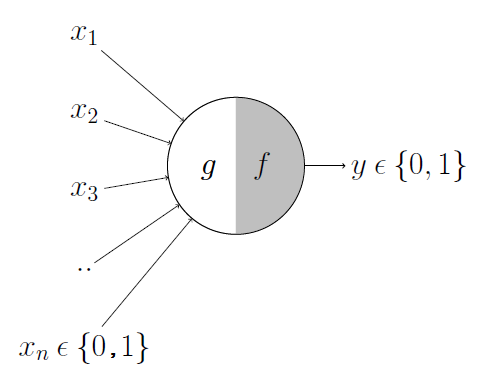
\includegraphics[width=0.8\textwidth]{images/mp.png}
    \caption{The threshold logic unit by McCulloch and Pitts. Source: \cite{med}}
    \label{fig:mp}
\end{figure}

A neural network arises when many of such artifical neurons are connected together. If the output of each neuron in one layer serves as the input to every neuron in the next layer (forming a complete bipartite graph) then these layers are called fully connected. When all the layers have this property, it is a fully connected neural network, such as the example in \autoref{fig:full}.\\

\begin{figure}
    \centering
    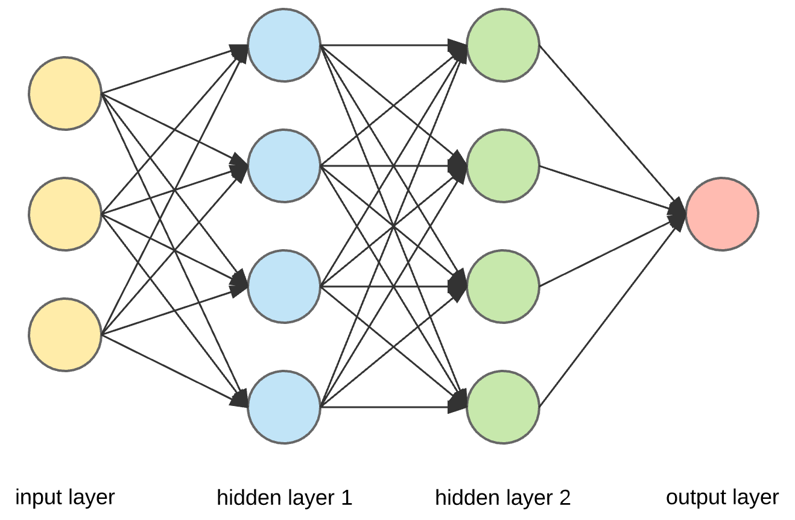
\includegraphics[width=0.8\textwidth]{images/fullyNet.png}
    \caption{An example of a fully connected neural network. Source: \cite{fullpic}}
    \label{fig:full}
\end{figure}

\subsection{Convolution}

Convolutional neural networks differ from regular neural networks in a couple of ways. First of all, they are much sparser in their connectivity, which means that a neuron is not influenced by all the neurons in the previous layer. However, particular neuron can still depend on all the values of a deeper layer indirectly, as shown in \autoref{fig:indir}.\\

\begin{figure}
    \centering
    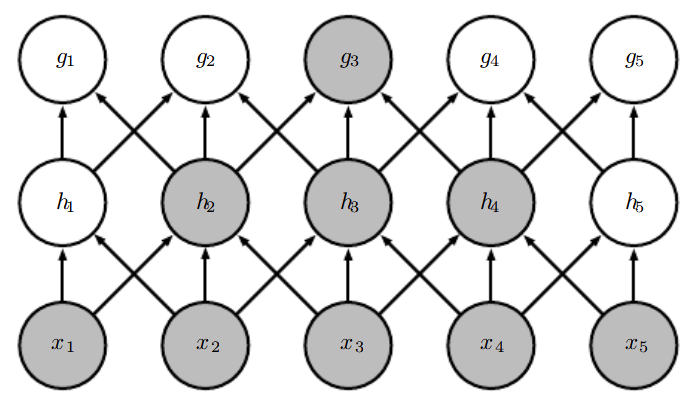
\includegraphics[width=0.8\textwidth]{images/indir.png}
    \caption{Neuron $g_3$ is indirectly influenced by all output values of a deeper layer. Source: \cite{dl-book}}
    \label{fig:indir}
\end{figure}

Another difference, from which ConvNets derive their name, is the fact that ConvNets use the convolution operation instead of regular matrix multiplication. We will go deeper into this topic in \autoref{sec:math}. A neural network is called convolutional, if at least one of its layers uses the convolution operation \cite[Ch. 9]{dl-book}.\\
%% eerst nog een stukje over hoezo regular matrix multiplication

There can still be some fully connected layers in a ConvNet, and actually this typically happens near the end of the network. For example, a ConvNet that is used to classify an image into the right category benefits from the fully connected layers to decifer the meaning of the feautures that the convolutional layers have extracted from the image. See \autoref{fig:typ}.

\begin{figure}
    \centering
    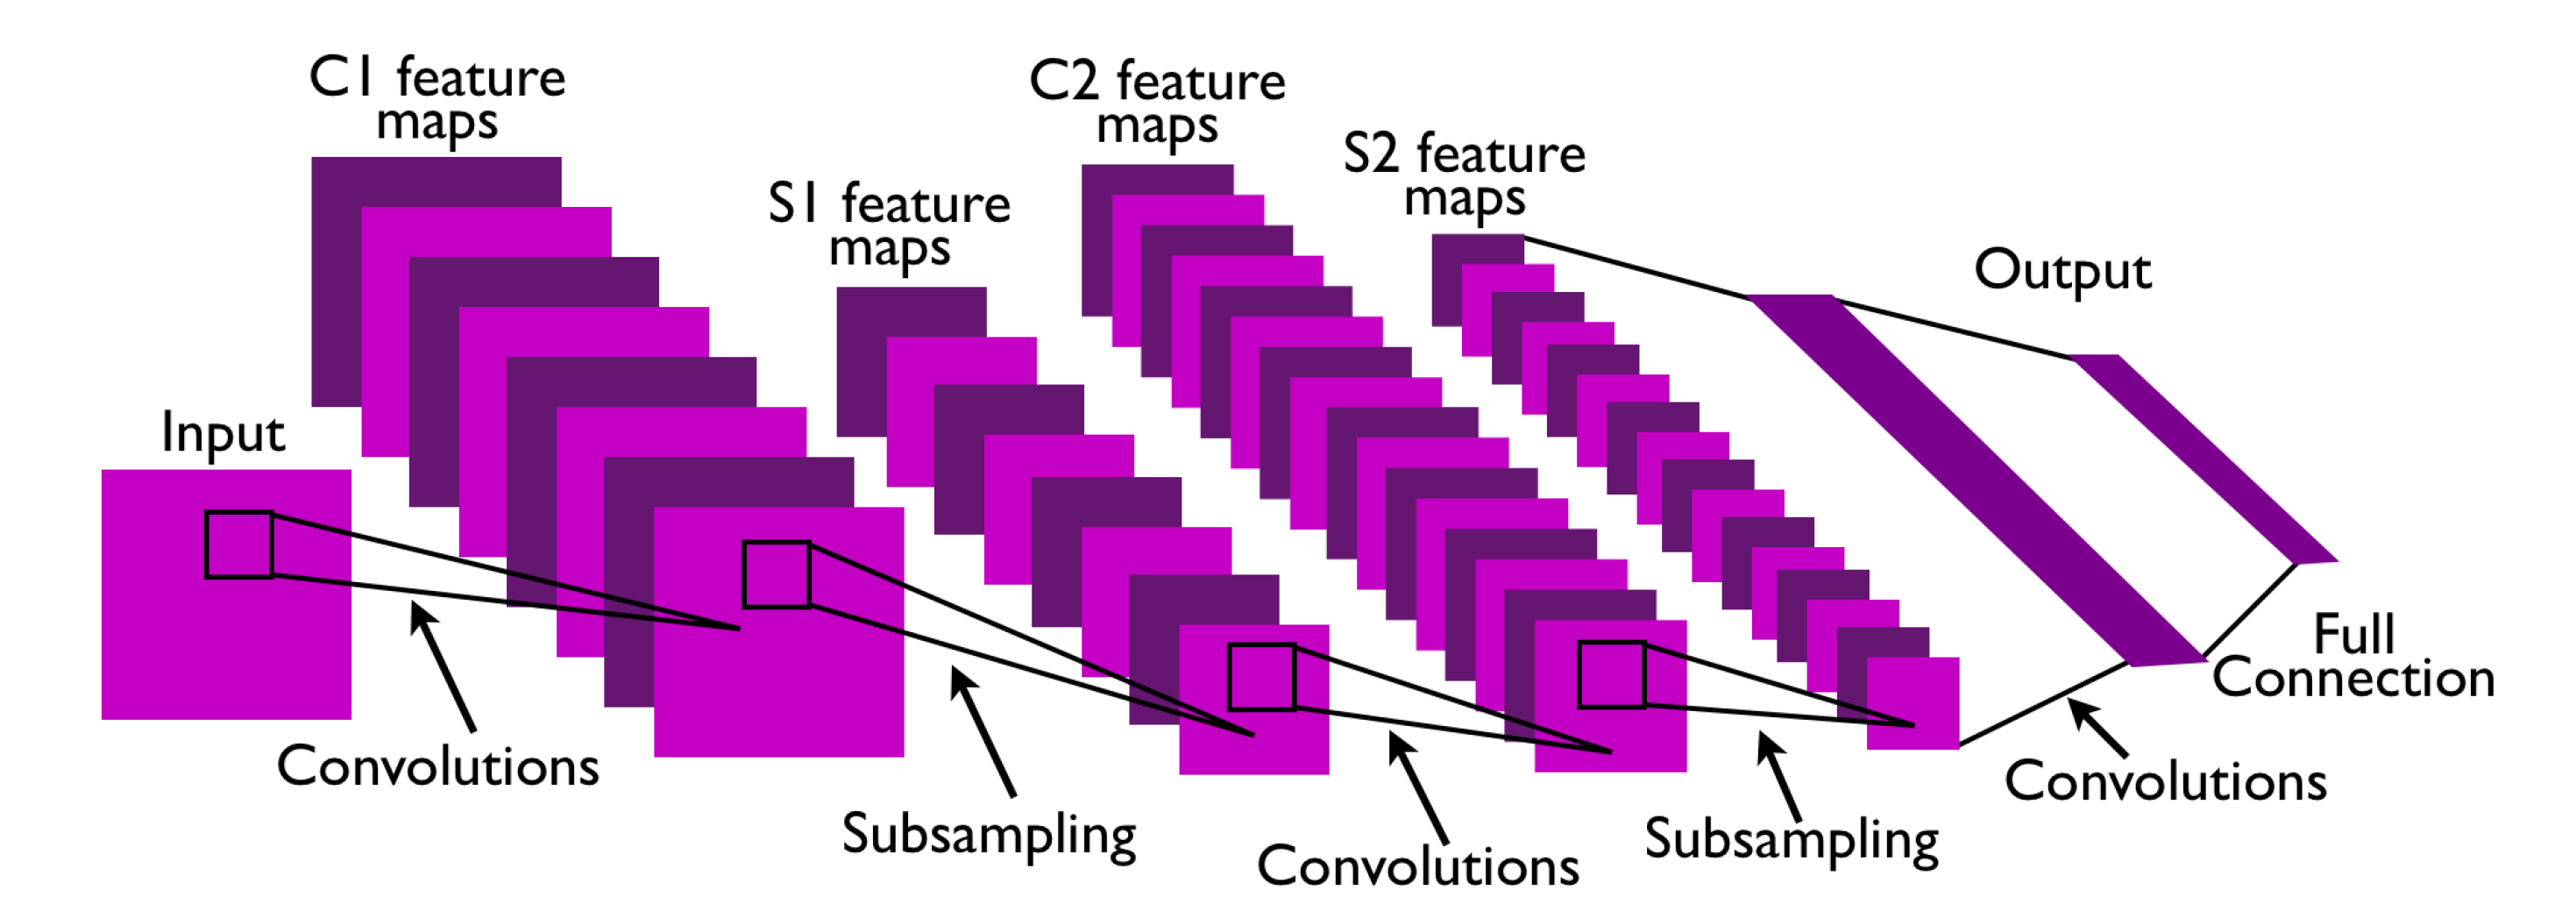
\includegraphics[width=\textwidth]{images/typicalConvNet.png}
    \caption{A typical ConvNet architecture. Source: \cite{convnet}}
    \label{fig:typ}
\end{figure}






